%--------------------------------------------------------------------------
%
%                                                    ENONCE
%
%--------------------------------------------------------------------------

\begin{center}
\vspace*{5mm}
\noindent {\Large {\bf Le manège à planche rétractable }}
\end{center}



\vspace*{10mm}
\begin{minipage}{0.5\textwidth}
Un manège est constitué d'un grand cylindre creux d'axe vertical ($Oz$) et de rayon R. Des personnes prennent place dans le cylindre, dos plaqué contre la face interne du cylindre et l'ensemble est mis en rotation à la vitesse angulaire $\vec\omega$. Lorsque la vitesse de rotation est suffisante, le plancher est retiré et les personnes restent ``collées à la paroi''.
\begin{enumerate}
\item Dans le référentiel tournant avec le manège, énumérer les forces exercées sur une personne à l'équilibre dans le manège. Quelle hypothèse sur les forces mises en jeu est nécessaire pour que l'équilibre soit possible ?
\item Si on note $\mu$ le coefficient de frottement statique avec la paroi, quelle est la vitesse minimale de rotation, $\omega_{\rm min}$, pour que le plancher puisse être retiré ?
\end{enumerate}
\end{minipage}
\hspace*{1cm}
\begin{minipage}{0.6\textwidth}
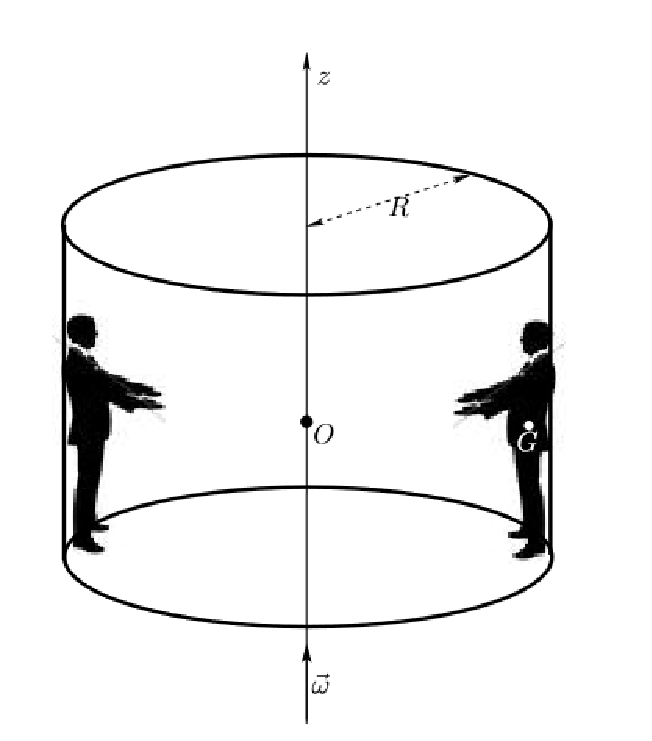
\includegraphics[width=7cm]{figures/serie14_fig1.pdf}
\end{minipage}\\

\emph{Indication: on fera l'approximation que le centre de masse de chaque personne se trouve à la distance $R$ de l'axe du cylindre.}
